\documentclass[border=0.2cm]{standalone}
\usepackage{tikz}
\usetikzlibrary{shapes.geometric}
 
\begin{document}
 
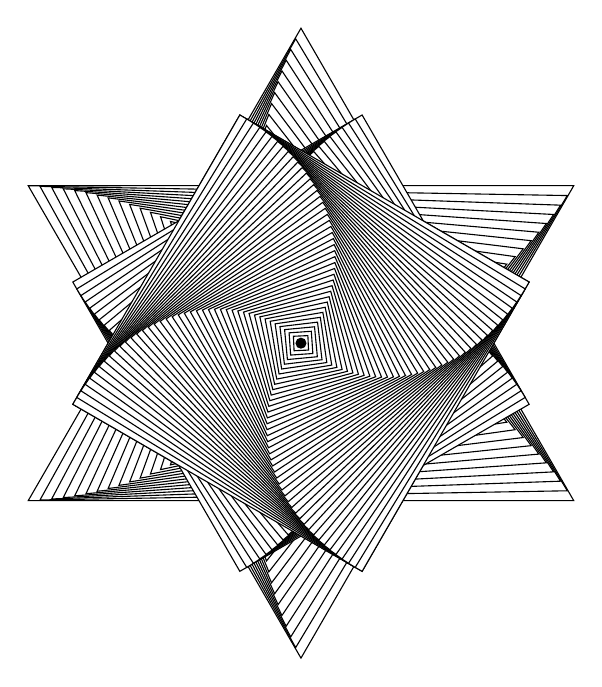
\begin{tikzpicture}[thin,black] 
\foreach \i in {-30,-29,...,0}{
 
\node[draw,
    fill=white!10,
    isosceles triangle,
    isosceles triangle apex angle=60,
    minimum size=-2*\i mm, 
    rotate=\i,inner sep =0pt] at (0,0){};
}

\foreach \i in {-30,-29,...,0}{
 
\node[draw,
    fill=white!10,
    isosceles triangle,
    isosceles triangle apex angle=60,
    minimum size=-2*\i mm, 
    rotate=-\i,inner sep =0pt] at (0,0){};
}

\foreach \i in {-30,-29,...,0}{
 
\node[draw,
    fill=white!10,
    regular polygon,
    regular polygon sides=4,
    minimum size=-2*\i mm, 
    rotate=-2*\i,inner sep =0pt] at (0,0){};
}

\foreach \i in {-30,-29.3,...,0}{
 
\node[draw,
    fill=white!10,
    regular polygon,
    regular polygon sides=4,
    minimum size=-2*\i mm, 
    rotate=90+2*\i,inner sep =0pt] at (0,0){};
}

\foreach \i in {-30,-29.3,...,0}{
 
\node[draw,
    fill=white!10,
    regular polygon,
    regular polygon sides=4,
    minimum size=-2*\i mm, 
    rotate=90-2*\i,inner sep =0pt] at (0,0){};
}

\fill (0,0) circle (2pt);

\end{tikzpicture}
 
\end{document}
